\hoofdstuk{Appendix I - Preliminary research}

\paragraaf{Appcelerator Titanium}
Appceleator Titanium is a commercially supported open source platform for developing cross-platform mobile applications. It was introduced by Appcelerator Inc in December 2008. Built upon the Eclipse IDE Titanium offers a Javascript API to native proxy classes which allow the developer to generate truly native cross-platform mobile applications. 

\subparagraaf{Platform support}
As of may 2012 Titanium supports iOS and Android. Next to building a native application for these platforms Titanium offers the option to generate a web application. 
Support for Research in Motion (BlackBerry) is in active (however closed from public) development. May first 2012 Appcelerator announced that it is extending its core value of cross-platform native application development beyond iOS and Android, on to RIM's BlackBerry devices.\cite{Asher2012}

\subparagraaf{Techniques and tools}
TitaniumStudio is an Eclipse based IDE with integration the proprietary mobile SDKs and simulators. For iOS this means Titanium requires Xcode with the iOS SDK to be installed, for Android the Android SDK and the Android AVD\footnote{AVD: Android Virtual Device (device simulator)} are required.

Titanium applications are written in JavaScript but can be augmented with HTML \& CSS. During runtime the JavaScript is evaluated and executed via so-called \emph{proxy objects}.Proxy Objects are objects which are paired to a native object and can resemble native user interface elements.\footnote{Proxy objects are discussed in more detail in chapter x:Proxy objects \   }.


\begin{centering}
	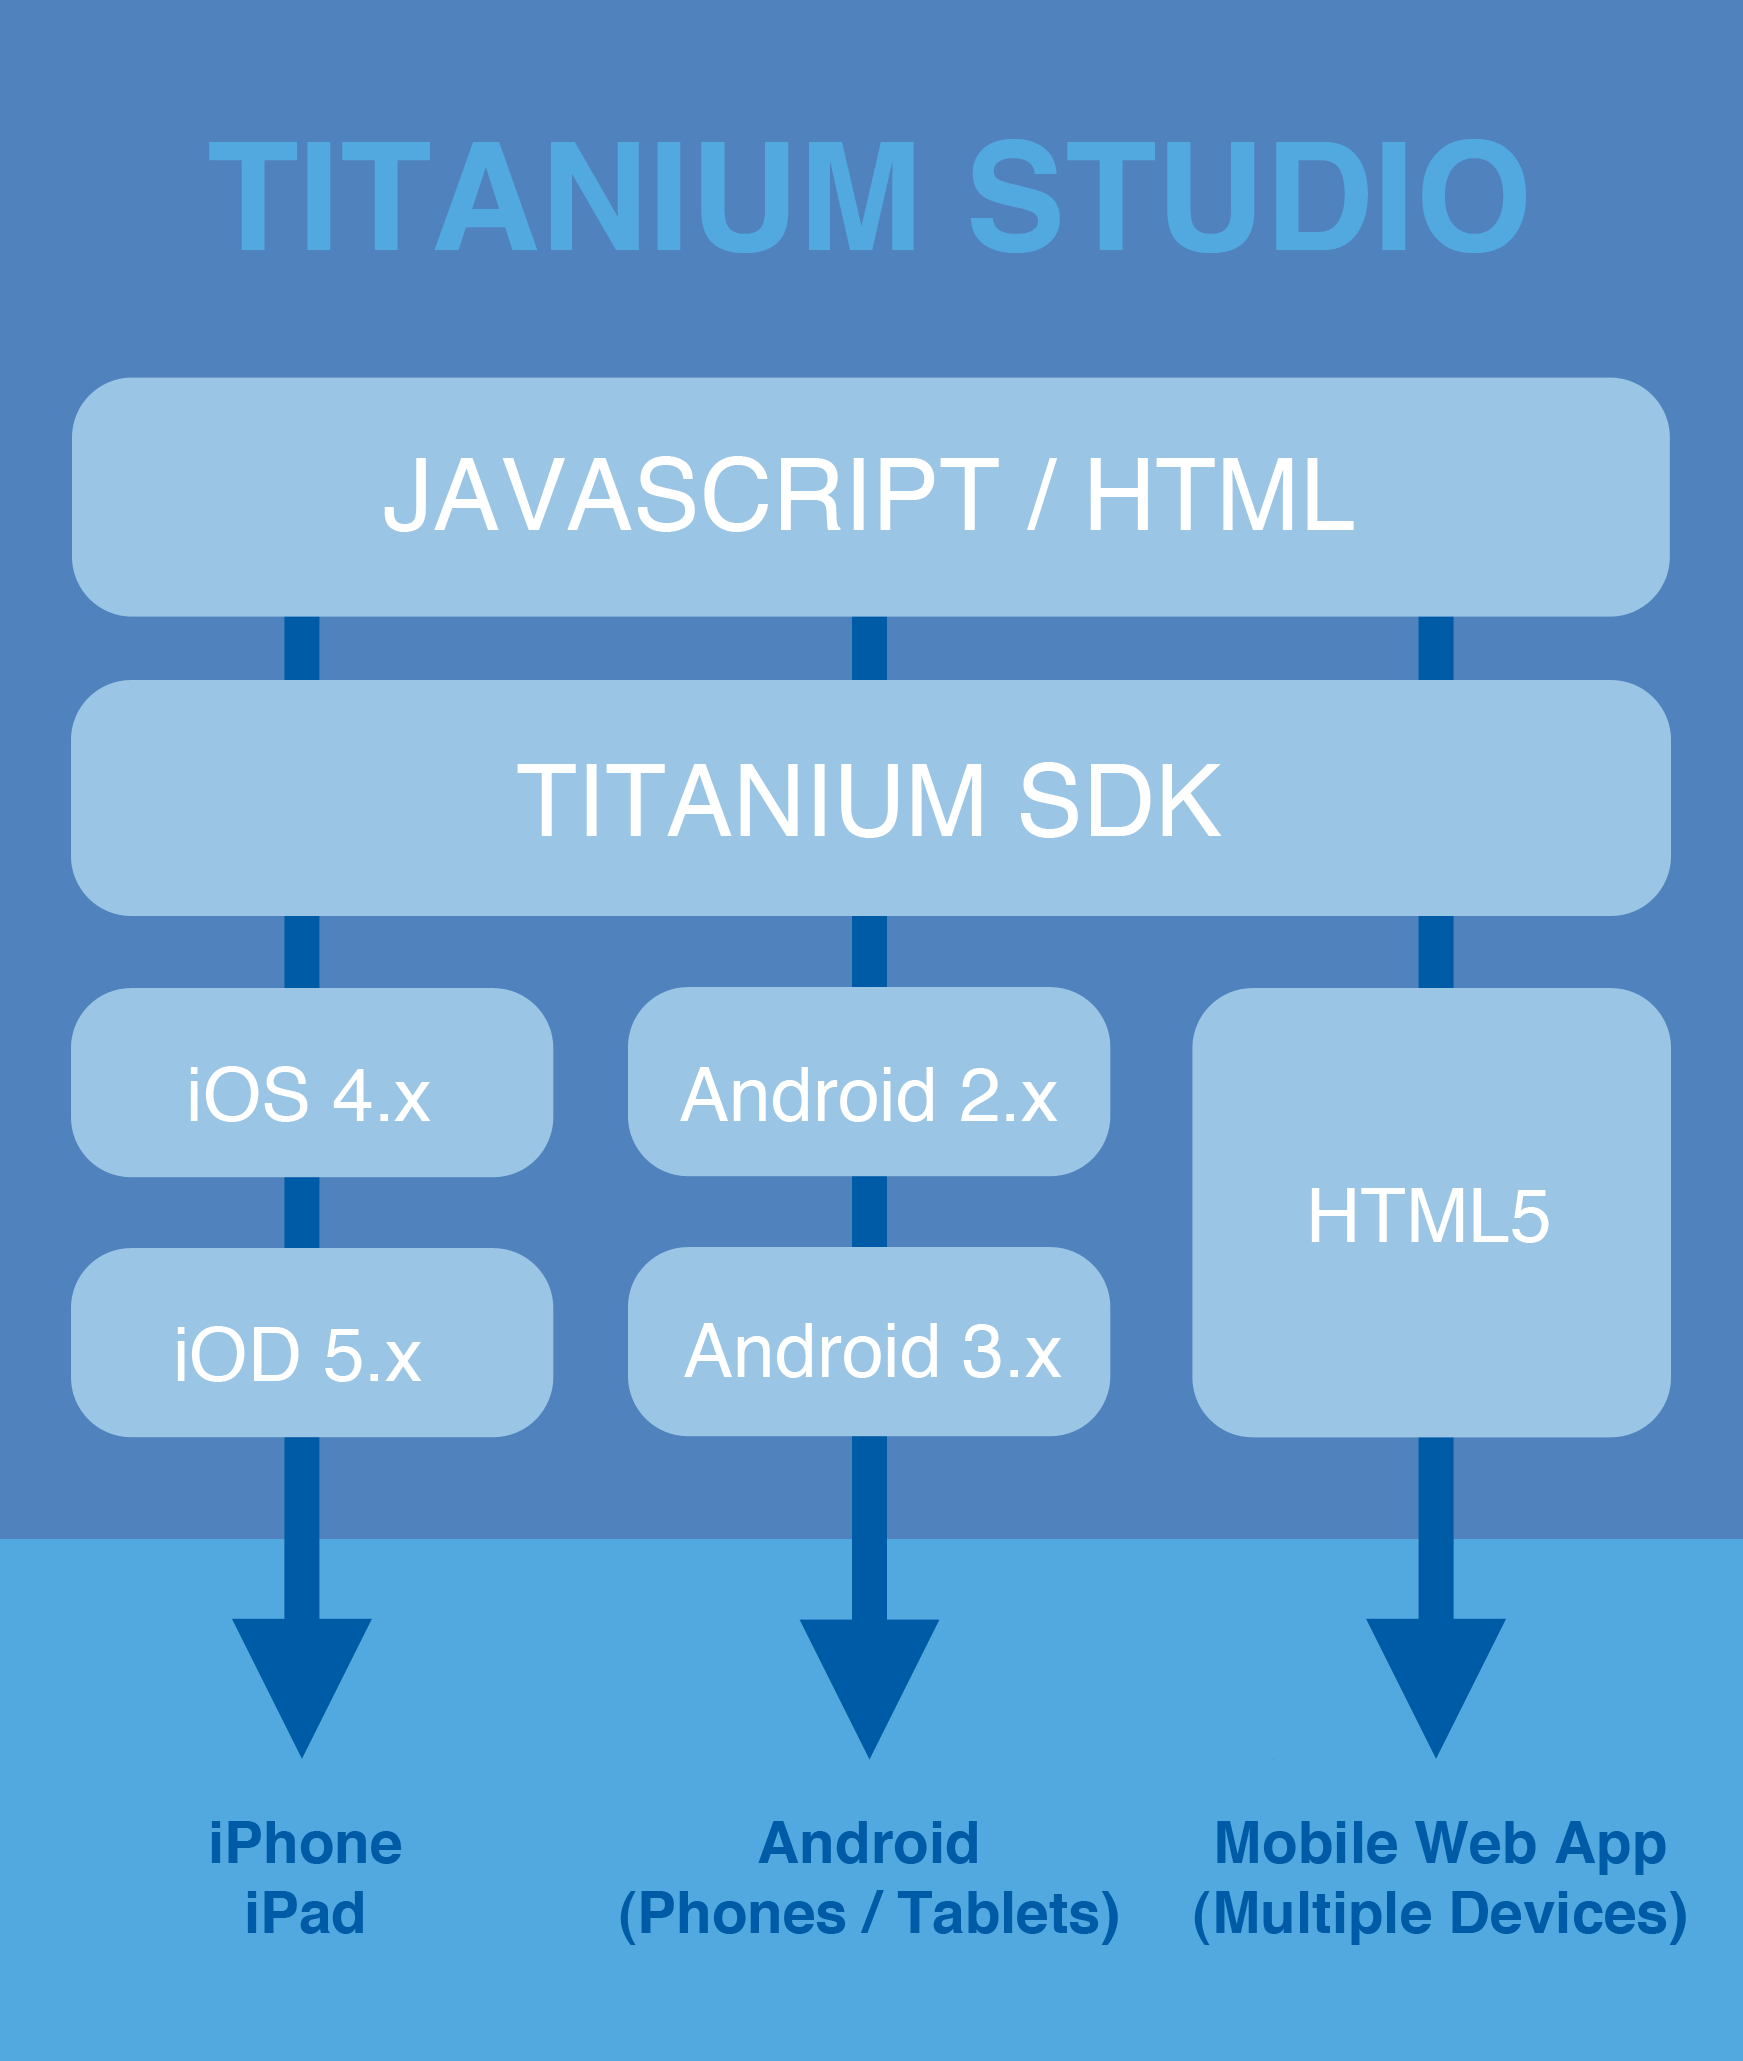
\includegraphics[scale=0.4]{images/titanium_architecture.png}\\{Titaniums bridge architecture\cite{Inc2012a}}\\
\end{centering}

\subparagraaf{Application type}
As mentioned above, Titanium applications are written in JavaScript but can be augmented with HTML \& CSS. The latter is in case a web application is required rather than a native application. This devices applications built with Titanium in two types:
\begin{itemize}
	\item
	Web applications
	\item
	Native applications
\end{itemize}

\subparagraaf{Philosophy}
The goal of Titanium is to provide a high level, cross-platform JavaScript runtime and API for mobile development.\cite{Whinnery2012} Titanium aims to help developers leverage their JavaScript knowledge to build native mobile apps that run across multiple platforms.

\subparagraaf{Results}
%todo aan elkaar hechten.

\begin{tabel}{ >\R p{\Procent{30}} | p{\Procent{60}} }{vbx}{Preliminary evaluation of Titanium}
\bf{Criteria} & \bf{Score}\\
 \hline
Platform support& ++\\
Native capabilities& +++\\
Programming language& JavaScript\\
IDE& Eclipse based studio\\
License type& Free but commercial available\\
Application type& Native\\
\end{tabel}

One of the issues which came up was that Titanium does not support DOM3 level specifications\cite{Whinnery2011}. This effectively rules out the x-path evaluate function which has support for an xml namespace resolver.\cite{Whitmer}

Finding this out took a while. I posted in Titaniums public Q\&A to no effect. I updated and closed the question myself after I found the cause of problem in Titaniums' documentation. \cite{Kraker2012a}\\

The original code, with a resolver function:

\begin{minted}[mathescape,
			   label="nsResolver",
               linenos,
               numbersep=5pt,
               gobble=0,
               frame=lines,
               framesep=2mm]{js}
function nsResolver(prefix) {
    var ns = {
        'atom' : 'http://www.w3.org/2005/Atom',
        'gd'   : 'http://schemas.google.com/g/2005'
    };
    return ns[prefix] || null;
}
var entries = doc.evaluate('//atom:entry', doc, nsResolver, XPathResult.ANY_TYPE, null);

\end{minted}

\noindent The solution is to use the predating DOM2 level xpath evaluate function:
\begin{minted}[mathescape,
			   label="DOM2",
               linenos,
               numbersep=5pt,
               gobble=0,
               frame=lines,
               framesep=2mm]{js}
var results = xml.evaluate("//*[local-name()='entry' 
		and namespace-uri()='"+ xml.namespaceURI+"']");
\end{minted}
Note that the function dates back to 2003 and prior. The namespace selection is hardcoded in the query, which is not very elegant.

\pagebreak

\paragraaf{Rhodes}
Rhodes is an ruby based open source framework developed by Motorola Rhodes. Rhodes focusses on the \emph{Modal View Controller} structure to seperate content from presentation. The views are written in HTML where as the controllers are to be written using Ruby. The Ruby is compiled into bytecode which is executed on the device. Each view is presented on the device’s browser rendering engine.

\subparagraaf{Platform support}
Rhodes supports iOS, Android, BlackBerry, Symbian, Windows Mobile

\subparagraaf{Techniques and tools}
Rhodes is an comes with an Eclipse based studio. Rhodes applications are primarily written using Ruby for business code and user interface control. For the actual user interface Rhodes relies on web techniques such as HTML, JavaScript and CSS. 
Rhodes focusses on the \emph{Model-View-Controller} pattern which is implemented using Ruby for the controllers and HTML for the views. The philosophy of the user interface is geared towards web technology using JavaScript libraries such as Sencha touch.

\subparagraaf{Application type}
Even though Rhodes advertises producing fully native apps\cite{RhoMobile}, they do not. In fact all they do is provide the user with a framework, access to some navigational user interface controls, but the rest of the user interface is html presented in a web-view. Although it is possible to augment the user interface with specific native components, it is not the focus of Rhodes.\\
\begin{centering}
	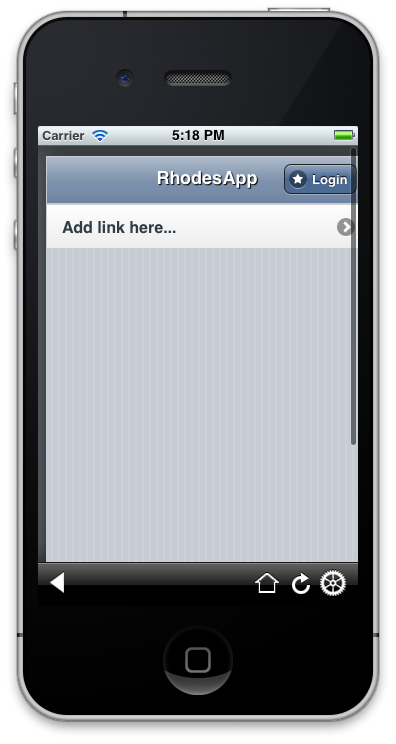
\includegraphics[scale=0.3]{images/rhodes_notsonative.png}\\{Rhodes iOS application: not very native}\\
\end{centering}

\subparagraaf{Philosophy}
Rhodes focusses on a user interface built with JavaScript libraries such as jQuery Mobile and Sencha, it is their believe that this creates a better user experience as native.\cite{Blum2011}

\subparagraaf{Results}
\begin{tabel}{ >\R p{\Procent{30}} | p{\Procent{60}} }{vbx}{Preliminary evaluation of Rhodes}
\bf{Criteria} & \bf{Score}\\
 \hline
Platform support& +++\\
Native capabilities& +-\\
Programming language& Ruby \& HTML, JavaScript and CSS\\
IDE& Eclipse based studio\\
License type& Free but commercial available\\
Application type& Framework hybrid applications\\
\end{tabel}

\pagebreak

\paragraaf{MoSync}
The MoSync mobile SDK offers cross-platform development trough the use of web technologies or C/C++.

\subparagraaf{Platform support}
MoSync supports Android, Java ME, iOS, Symbian and Windows Mobile.

\subparagraaf{Techniques and tools}
MoSync allows for development in C/C++ or HTML, CSS and Javascript. Plugins are offered for the Eclipse IDE and Visual studio. However when run in Visual Study MoSync cannot compile for iOS.

\subparagraaf{Application type}
Although some native user interface elements are usuable trough the MoSync SDK the number of these available elements is very small.\cite{Mosync2012} This leads to conclude that the native capabilities is still in a very early phase.  MoSync relies heavily at the use of web technologies for view generation, therefore MoSync produces webview-based hybrid applications. 

\subparagraaf{Philosophy}
The goal of MoSync is to provide an east and cost effective solution to develop and distribute mobile applications cross-platform trough the native distribution channels.

\subparagraaf{Results}
\begin{tabel}{ >\R p{\Procent{30}} | p{\Procent{60}} }{vbx}{Preliminary evaluation of MoSync}
\bf{Criteria} & \bf{Score}\\
 \hline
Platform support& ++\\
Native capabilities& -\\
Programming language&  C++ \& HTML, CSS and Javascript\\
IDE& Eclipse plugin, Visual Studio plugin\\
License type& Free\\
Application type& Webview-based hybrid applications\\
\end{tabel}

\pagebreak

\paragraaf{Worklight}
Worklight Studio is an eclipse based IDE for the cross-platform development of mobile applications. Worklight Studio was introduced in 200x by Worklight Inc. In early 2012 Worklight Inc. became an IBM company. Worklight Studio offers mobile development trough the use of web technologies such as HTML, and Javascript.

Worklight advertises the capability for developers to develop crossplatform HTML5, hybrid and native mobile applications.


\subparagraaf{Platform support}
Worklight supports the following platforms: iOS, Android, BlackBerry and Windows Mobile 7.

\subparagraaf{Techniques and tools}
As mentioned above, Worklight Studio is an eclipse based IDE.
Allows the developer access to device APIs using native code or standard HTML5, CSS3 and JavaScript over a uniform PhoneGap bridge.


\subparagraaf{Application type}
Applications developed with Worklight can be classied as \emph{Webview-based hybrid applications}. As defined in the previous chapter this means the applications are based fitted inside web-view and build on a framework which provides an API to allow the application access to otherwise native API's. The latter is achieved trough Worklights SDK while the former is made possible by an implementation of PhoneGap. \cite{Inc2012}

\begin{centering}
  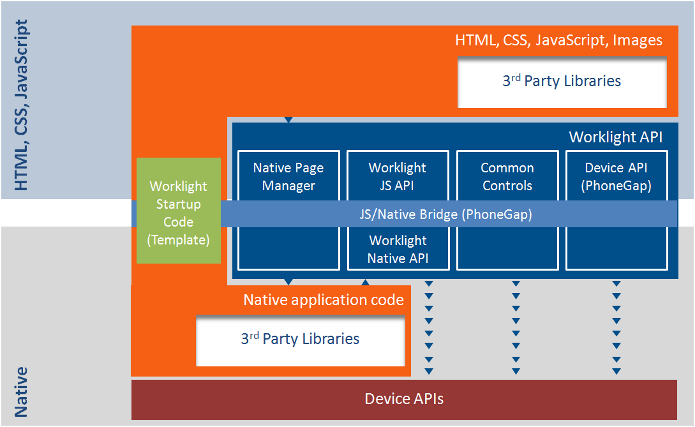
\includegraphics[scale=0.5]{images/Worklight_architecture.png}\\{Worklights bridge architecture\cite{Inc2012a}}\\
\end{centering}

\subparagraaf{Philosophy}
Worklight aims to grant developers access trough HTML5 to the capabilities that mobile devices provide. 

\subparagraaf{Results}

\begin{tabel}{ >\R p{\Procent{30}} | p{\Procent{60}} }{vbx}{Preliminary evaluation of Worklight}
\bf{Criteria} & \bf{Score}\\
 \hline
Platform support& ++\\
Native capabilities& -\\
Programming language&  HTML, JavaScript and CSS\\
IDE& Eclipse based studio with PhoneGap integration\\
License type& Commercial\\
Application type& Webview-based hybrid applications\\
\end{tabel}